\section{The algorithm} \label{sec:algorithm}

%%%%%%%%%%%%%%%%%%%%%%%%%%%%%%%%%%%%%%%%%%%%%%%%%%%%%%%%%%%%%%%%%%%%%%%%%%%%%%%%%%
%%%%%%%%%%  OVERVIEW
%%%%%%%%%%%%%%%%%%%%%%%%%%%%%%%%%%%%%%%%%%%%%%%%%%%%%%%%%%%%%%%%%%%%%%%%%%%%%%%%%%
\subsection{Overview} \label{sec:algorithm:overview}
The Omicron algorithm is developed in C++ and the code lives in the Virgo software repository~\cite{VirgoSVN}. Omicron is built upon GWOLLUM~\cite{GWOLLUM} libraries used to perform every step of an Omicron analysis (see Fig.~\ref{fig:omicron_incl} for a dependency diagram). The GWOLLUM package depends on external libraries. The FrameL~\cite{FrameL} library is used to perform IO operations on data frame files~\footnote{The frame format was developed for interferometric gravitational-wave detectors' data.}. Mathematical routines developed in the GNU Scientific Library~\cite{GSL} are commonly used by GWOLLUM functions. Discrete Fourier transforms are performed using the FFTW~\cite{FFTW} algorithm. Finally, the GWOLLUM and Omicron codes heavily rely on C++ classes developed in the ROOT~\cite{Brun:1997pa} framework. For example, ROOT classes are used for plotting purposes, for event storage or for data access. To deal with package dependencies, the CMT~\cite{CMT} configuration management tool was chosen.

A fully object-oriented framework is adopted when developing GWOLLUM and Omicron, in which C++ classes and inheritance features are extensively used. The Omicron algorithm is entirely based on the \texttt{Omicron} C++ class which member functions are used to perform the analysis steps. A typical Omicron application can be represented by the sequence of functions represented in Fig.~\ref{fig:omicron_flowchart}. The \texttt{Omicron} constructor must be called using an input option file listing all the parameters defining the search one wants to perform. Then, the Omicron object must be provided with time segments to process. This is done with the \texttt{Omicron::InitSegment()} function. These time segments are processed sequentially with the \texttt{Omicron::NewChunk()} function. For every chunk, the list of channels to process is looped over with the \texttt{Omicron::NewChannel()} function. The input data is loaded with the \texttt{Omicron::LoadData()} function. The data is then conditioned; it is down-sampled to a working frequency and high-pass filtered. This is performed with the  \texttt{Omicron::Condition()} function. Before applying the Q-transform, the data is whitened by normalizing the data spectrum by the noise power spectrum density. The whitened data is finally projected onto a basis of windowed complex exponentials. This is done using the \texttt{Omicron::Project()} function. When calling the \texttt{Omicron::WriteOutput()} function, the Omicron data products are saved to disk\footnote{The html report is saved when calling the \texttt{Omicron} destructor.}.

\begin{figure}
  \center
  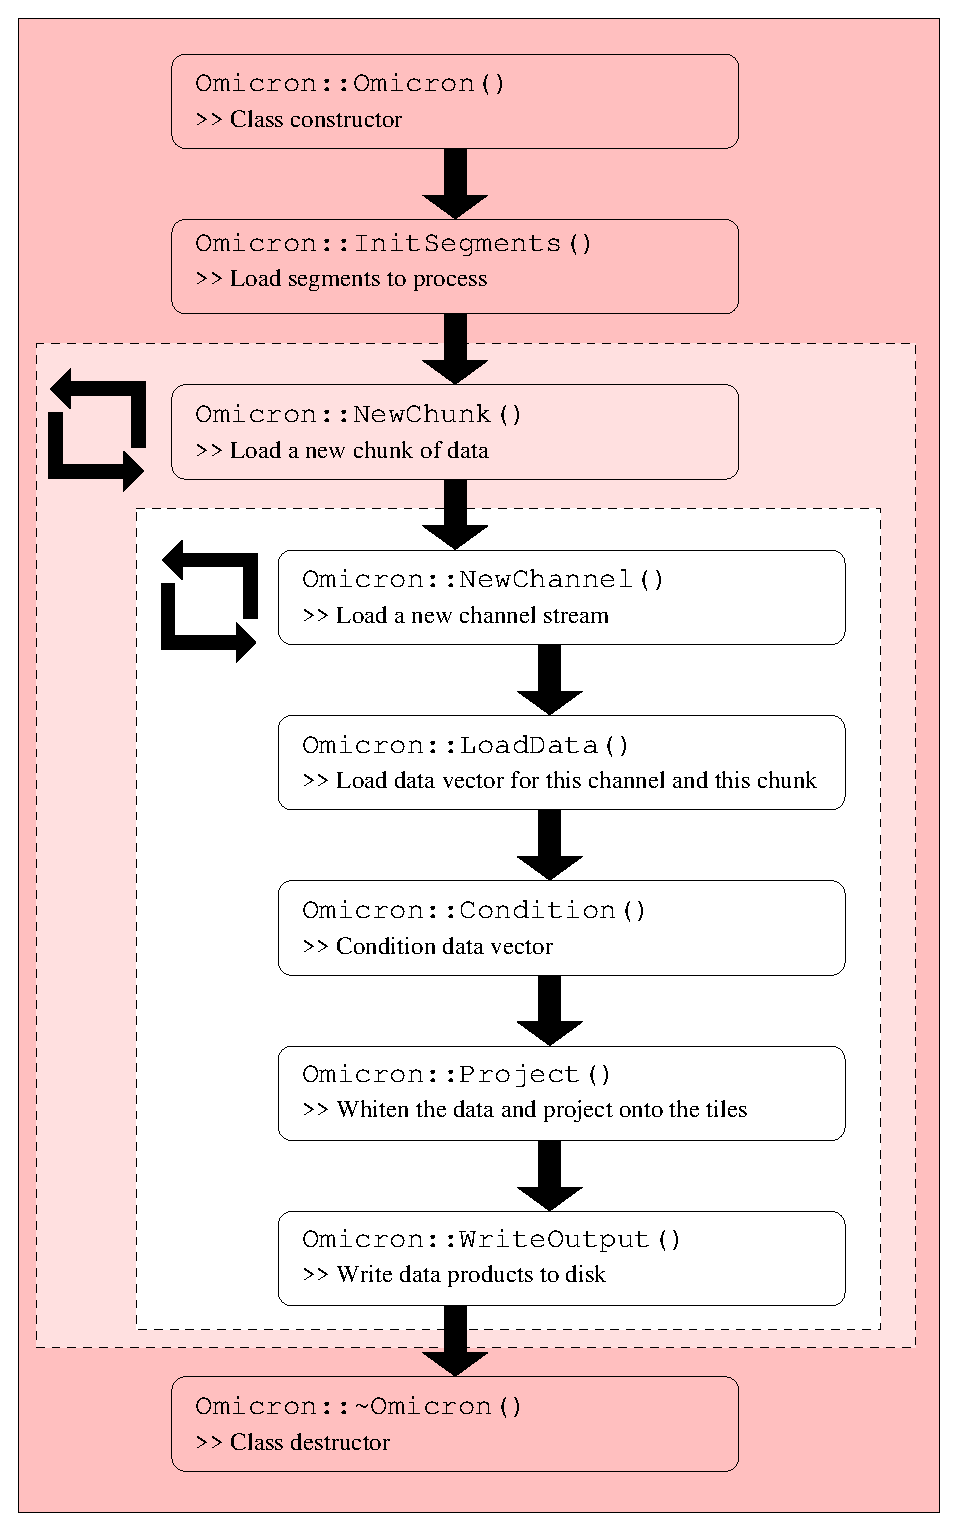
\epsfig{width=10cm, file=./figures/omicron_flowchart.eps}
  \caption{Standard \texttt{Omicron} flowchart. The standard sequence of class functions is presented. Loops must be perfomed over data chunks and channels. They are represented by the pink rectangles.}
  \label{fig:omicron_flowchart}
\end{figure}

This sequence of actions is performed by the \texttt{omicron.exe} executable. This programs runs the Omicron analysis using a list of arguments:
\begin{itemize}
  \item \texttt{omicron.exe gps\_start gps\_stop /path/to/parameters.file}. The Omicron algorithm is run over a single time segment starting at GPS time \texttt{gps\_start} and stopping at GPS time \texttt{gps\_end} and using the parameters listed in the file \texttt{/path/to/parameters.file}.
  \item \texttt{omicron.exe /path/to/segments.file /path/to/parameters.file}. The Omicron algorithm is run over all the time segments listed in \texttt{/path/to/segments.file} and using the parameters listed in the file \texttt{/path/to/parameters.file}.
  \item \texttt{omicron.exe gps\_center /path/to/parameters.file}. The Omicron algorithm is run over a single time chunk centered on GPS time \texttt{gps\_center} and using the parameters listed in the file \texttt{/path/to/parameters.file}.
\end{itemize}
The \texttt{Omicron} class offers more methods which can be used to tailor specfic application. For an up-to-date and extensive description of these methods, refer to the doxygen documentation~\cite{Omicron_doxygen}.

\begin{figure}
  \center
  \includegraphics[angle=90, scale=0.4]{./figures/omicron_incl}
  \caption{Diagram presenting the Omicron code dependencies. Header files starting with a ``O'' are part of the Omicron Package. Header files starting with a ``T'' are taken from the ROOT~\cite{Brun:1997pa} libraries. \bluenote{Clean this!}}
  \label{fig:omicron_incl}
\end{figure}

%%%%%%%%%%%%%%%%%%%%%%%%%%%%%%%%%%%%%%%%%%%%%%%%%%%%%%%%%%%%%%%%%%%%%%%%%%%%%%%%%%
%%%%%%%%%%  DATA ACCESS
%%%%%%%%%%%%%%%%%%%%%%%%%%%%%%%%%%%%%%%%%%%%%%%%%%%%%%%%%%%%%%%%%%%%%%%%%%%%%%%%%%
\subsection{The data access} \label{sec:algorithm:data}
The input data time series is read using the FrameL~\cite{FrameL} library, developed to perform read/write file operations using the Frame format\footnote{The frame format is a data format specifically developed for interferometric gravitational-wave detectors.}. The data must be provided through a Frame File List (FFL) file which consists in an ASCII file with the file extension ``.ffl''. This file must contain a list of frame files described over five columns: the path to the frame file, the GPS information for the file start, the file duration in seconds, the GPS time of the first event and the GPS time of the last event\footnote{A FFL file can be obtained using the FrameL program \texttt{FrDump.exe}: \texttt{FrDump.exe -i /path/to/frame/files/*.gwf -d 0 $>$ fflfile.ffl}}. The GWOLLUM class, \texttt{ffl}, was designed to offer an improved C++ interface to access frame data. For example, the \texttt{ffl} class provides compatibility with the specific LIGO lal-cache file format.

The \texttt{ffl} class is used by Omicron to load data by time chunks. The \textit{chunk} is an important charactistic time scale which is user-defined in the parameter file. It defines the time sequence adopted to analyze the data. It is also used as a characteric time scale by many Omicron internal structures; the chunk duration (which we note $T_c$) directly impacts the tiling resolution, determines the output files size, and is used to allocate memory for data containers.

Fig.~\ref{fig:segmentation} presents how the input data is segmented and analyzed. The input time segments, provided by the Omicron command line, are subdivided into chunks. The size of the chunks is fixed and is defined in the user parameter file. Chunks overlap by a fixed amount of time. The overlap duration is also defined in the user parameter file. The segment size does not generally matches the chunk and overlap structure. As a result, for the last chunk, the overlap is adjusted to fit the segment size. The overlapping structure was introduced to manage edge artifacts due to forward and backward filtering of the data (see Sec.~\ref{sec:algorithm:conditioning}). Some data is irremediably lost in this process: segments shorter than the chunk duration cannot be analyzed and the first and last edges of a segment (half the overlap) are not saved.
\begin{figure}
  \center
  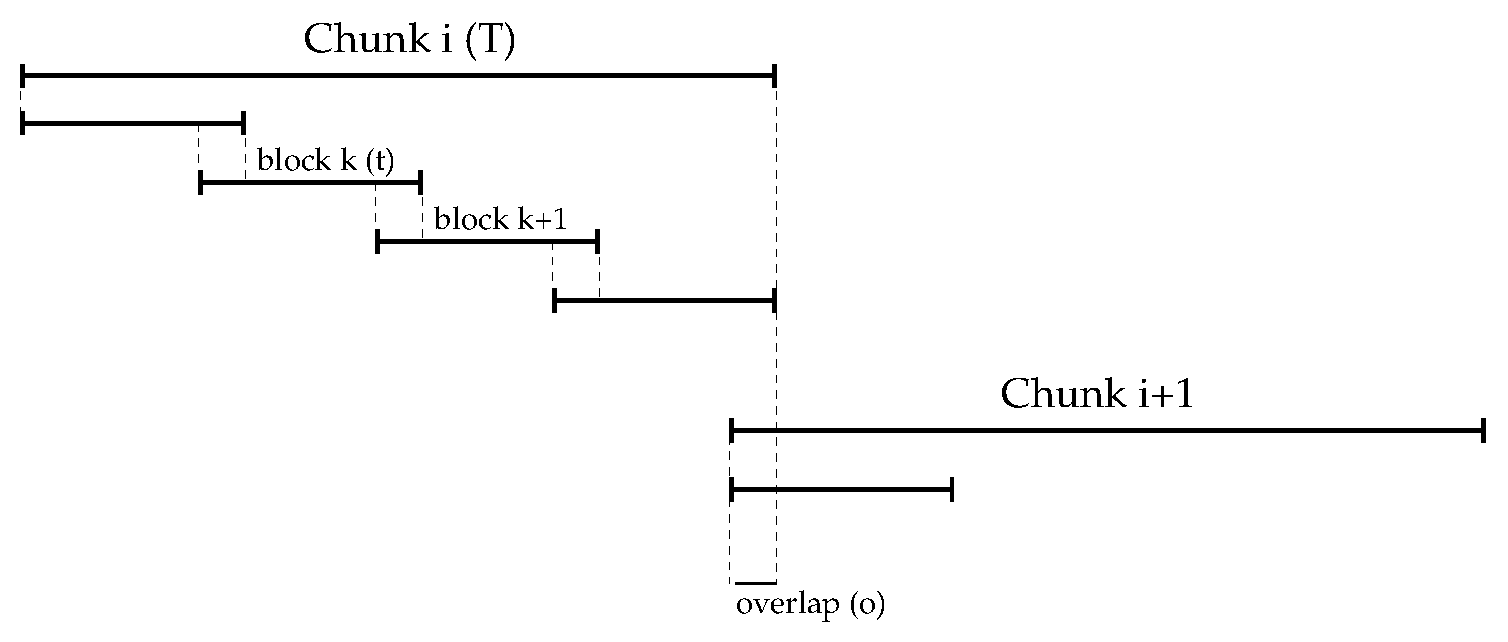
\epsfig{width=15cm, file=./figures/segmentation.eps}
  \caption{Data segmentation. The input segments are analyzed sequentially, chunk by chunk. The chunks, represented by the red lines, have a fixed size and are defined in the user parameter file. They overlap by a fixed amount of time, also defined in the parameter file. The overlap for the last chunk of a segment is modified to adjust the segment size. Only the central part of the chunk, represented by the black lines, is meaningful. Only Omicron triggers in this central region are saved.}
  \label{fig:segmentation}
\end{figure}

The chunk and overlap structure must verify some conditions:
\begin{enumerate}
\item The durations must be integer values. Omicron only supports integer durations.
\item The chunk duration must be a power of 2 value and longer than or equal to 4 seconds. This is required to construct the tiling structure, refer to Sec.~\ref{sec:algorithm:tiling}.
\item The overlap duration must be an even value and shorter than the chunk duration for obvious reasons.
\end{enumerate}

For a given chunk and a given channel\footnote{Chunks and channels are internally looped over using the \texttt{Omicron::NewChunk()} and \texttt{Omicron::NewChannel()} functions.}, a chunk data vector is filled with the raw time series. The native sampling frequency for this channel data stream, $f_s$ is directly given by the size of the vector and is checked for evey chunk. This way, a change of the channel sampling frequency is automatically accounted for when looping over the chunks.


%%%%%%%%%%%%%%%%%%%%%%%%%%%%%%%%%%%%%%%%%%%%%%%%%%%%%%%%%%%%%%%%%%%%%%%%%%%%%%%%%%
%%%%%%%%%%  DATA CONDITIONING
%%%%%%%%%%%%%%%%%%%%%%%%%%%%%%%%%%%%%%%%%%%%%%%%%%%%%%%%%%%%%%%%%%%%%%%%%%%%%%%%%%
\subsection{The data conditioning} \label{sec:algorithm:conditionnig}
The chunk data vector is transformed to optimize the performance of the subsequent processing. It is down-sampled to a lower working frequency, $f_w$, to maximize the processing speed and lower the memory usage. It is then high-pass filtered to reduce the signal dynamic range. The filtering C++ code is inspired from the routines developed in the LSC Algorithm Library Suite~\cite{LALSUITE}.

To avoid aliasing, a 20$^{\mathrm{th}}$-order Butterworth low-pass filter with an attenuation factor of 0.1 is applied using a cutoff frequency set at the targeted Nyquist frequency, $f_w/2$. The filter is applied in the time domain first forwards and then backwards in order to cancel the phase delay introduced by a single pass. The disadvantage of the Butterworth filter is that since it is an IIR filter, it is not possible to determine the exact length of corrupted data at the start and end of the output time series. The chunk overlap duration (see, Sec.~\ref{sec:algorithm:data}) must be chosen with care to reject these filtering artifacts. Finally, the time-series is decimated to the desired working sampling frequency. The resulting working data vector size is now reduced to $f_w \times T_c$.

The working vector is high-pass filtered using a 12$^{\mathrm{th}}$-order Butterworth filter.

\begin{figure}
  \center
  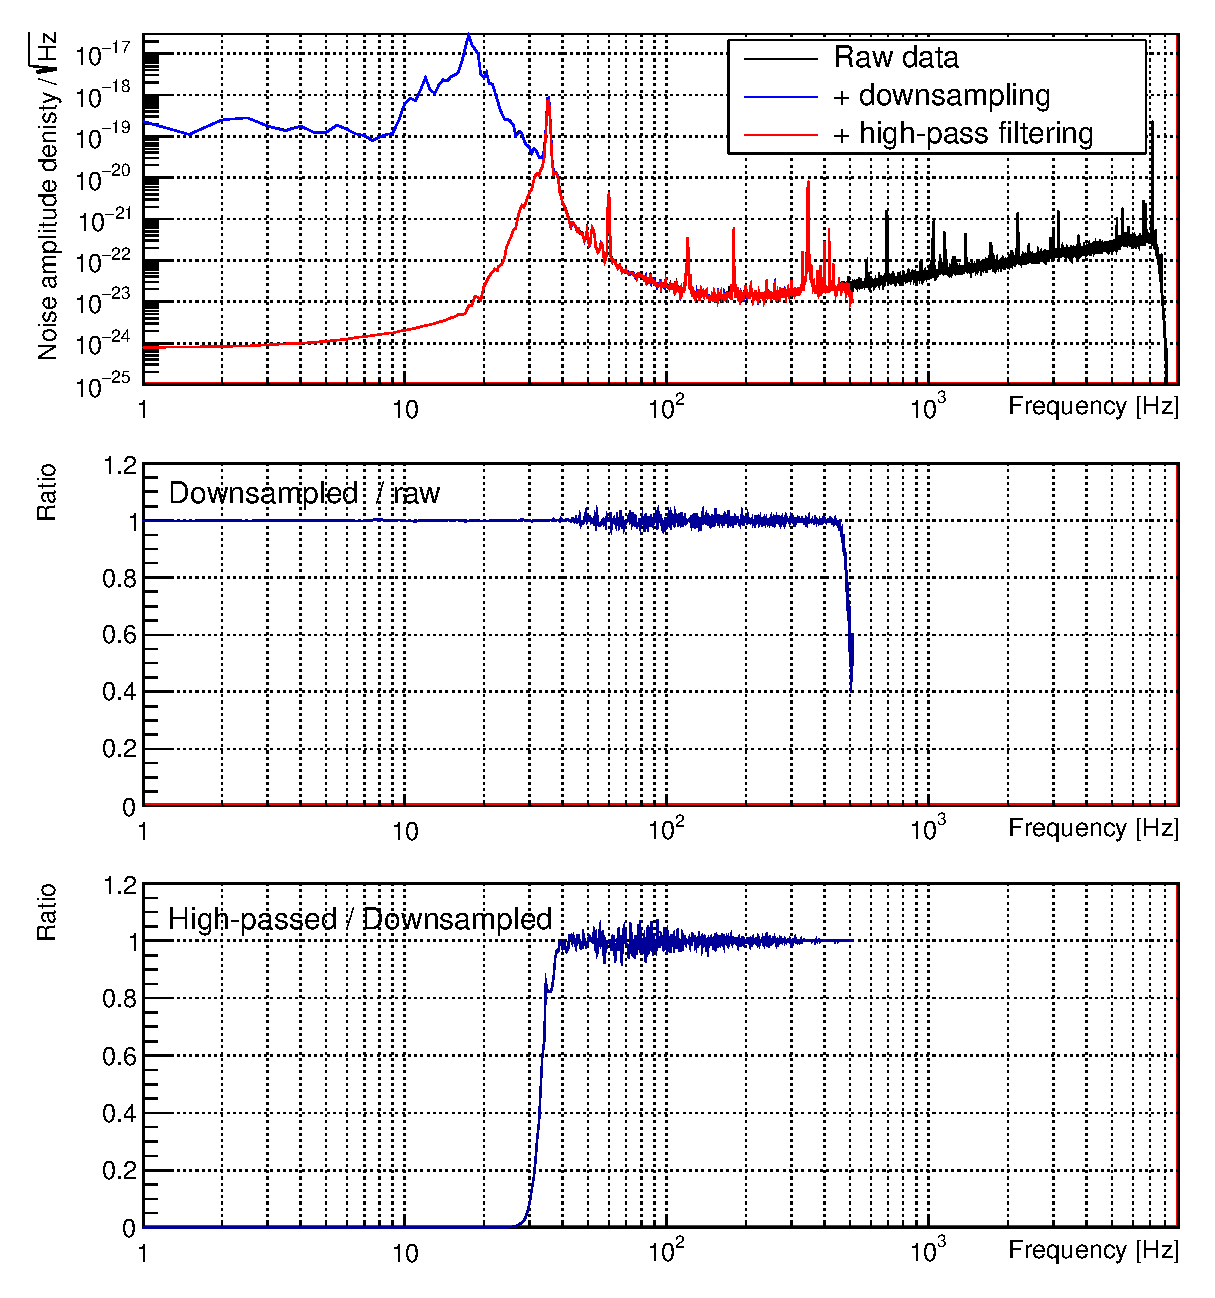
\epsfig{width=10cm, file=./figures/conditioning.eps}
  \caption{The upper plot displays the noise data spectra measured at different steps of the conditioning process. The black curve presents the spectrum of the raw data between 1~Hz and the Nyquist frequency of 8192~Hz. The raw data are downsampled to a working frequency $f_w=1024$~Hz. The resulting spectrum is represented in blue. The downsampled data is then high-pass filtered ($f>40$~Hz) and the measured spectrum is represented in red. The ratio between the downsampled and the raw spectrum is plotted in the middle. The lower plot shows the ratio between the high-passed and the downsampled spectra. }
  \label{fig:conditioning}
\end{figure}



%%%%%%%%%%%%%%%%%%%%%%%%%%%%%%%%%%%%%%%%%%%%%%%%%%%%%%%%%%%%%%%%%%%%%%%%%%%%%%%%%%
%%%%%%%%%%  DATA WHITENING
%%%%%%%%%%%%%%%%%%%%%%%%%%%%%%%%%%%%%%%%%%%%%%%%%%%%%%%%%%%%%%%%%%%%%%%%%%%%%%%%%%
\subsection{The data whitening} \label{sec:algorithm:whitening}
- PSD definition - PSD implementation (size, FT...).

To obtain a reliable PSD estimation, we use the procedure defined in~\cite{psd}.
The data chunk is divided into N segments overlapping by half, as represented in Fig.~\ref{fig:mmm}. The PSD of each segment is computed. This set of PSDs is divided into two groups corresponding to non-overlapping segments: the 'odd' (resp. 'even') group is defined with segments with an odd (resp. even) index.
\begin{figure}
  \center
  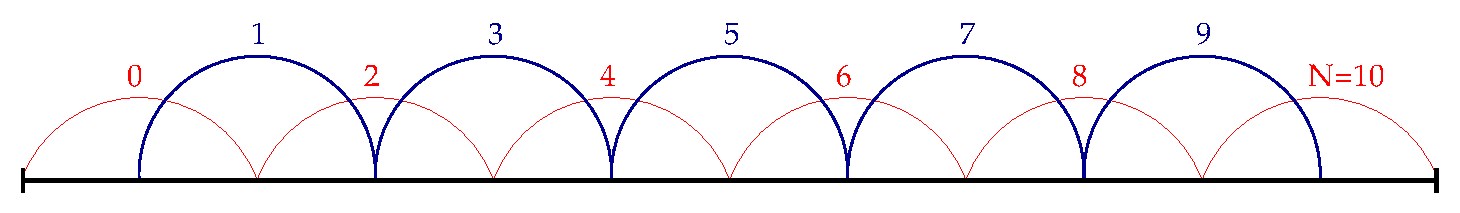
\epsfig{width=15cm, file=./figures/mmm.eps}
  \caption{Power spectral density estimation. The data chunk is divided into.}
  \label{fig:mmm}
\end{figure}


\subsection{The tiling} \label{sec:algorithm:tiling}

\subsection{The filtering} \label{sec:algorithm:conditioning}

\subsection{The triggering} \label{sec:algorithm:triggering}

\subsection{The clustering} \label{sec:algorithm:conditioning}

\subsection{The mapping} \label{sec:algorithm:mapping}
